\documentclass{IEEEcsmag}

\usepackage[colorlinks,urlcolor=blue,linkcolor=blue,citecolor=blue]{hyperref}

%\usepackage{upmath}
\usepackage{xspace}
\usepackage{graphicx}
%\usepackage[version=3]{mhchem}
%\usepackage{bm}
%\usepackage{siunitx}
%\usepackage{natbib}

\newcommand*{\kovats}{Kov\'ats\xspace}

\jvol{XX}
\jnum{XX}
\paper{8}
\jmonth{May/June}
\jname{IT Professional}
\pubyear{2019}
\newtheorem{theorem}{Theorem}
\newtheorem{lemma}{Lemma}

\setcounter{secnumdepth}{0}

\begin{document}

\sptitle{Department: Head}
\editor{Editor: Name, xxxx@email}

\title{Predicting Retention Indices of Chemical Compounds Using Graph Neural Network}

\author{Chen Qu}
\affil{Applied and Computational Mathematics Division, National Institute of Standards and Technology, 100 Bureau Drive, Gaithersburg, Maryland 20899, USA and Department of Chemistry \& Biochemistry, University of Maryland, College Park, Maryland 20742, USA}

%\author{S. B. Author, Jr.}
%\affil{Second Affiliation}

\markboth{Department Head}{Predicting Retention Indices of Chemical Compounds Using Graph Neural Network}

\begin{abstract}
The \kovats retention index is a system-independent quantity that characterizes the rate at which a compound is processed through a gas chromatography column. The capability to precisely predict this quantity could lead to a more reliable and efficient scheme for compound identification. We have trained a graph convolutional neural network model using a database maintained by NIST, and predict the \kovats retention index with a mean unsigned error of 28 index units as compared to 114 from the estimation scheme currently incorporated in the database. The results convincingly demonstrate the predictive powers of systematic, data-driven approaches applied to chemical data.
\end{abstract}

\maketitle

% background about GC and MS
\chapterinitial{Gas chromatography} (GC) is an important analytical technique for the separation and identification of chemical compounds. In a GC experiment, a mixture of unknown substances in gaseous state is passed through a chromatography column and compounds in the mixture are separated. It has been demonstrated\cite{1958Kovats} that the retention time of a compound (the time it takes to pass through the column) could be converted to a dimensionless quantity that is independent of many experimental factors such as column length and diameter. This quantity is the \kovats retention index (KRI), and it could be used for identifying compounds.

However, KRI alone is usually not sufficient for a precise identification, so GC is frequently used in combination with mass spectrometry (GC/MS) to enhance the accuracy of the identification, by matching both the KRI and mass spectrum against those in a library of measured compounds. This two-step process considerably improves the confidence of the identification scheme.
Thus, there is significant value in developing an accurate predictive model for the KRI.

The rapid advances in machine learning, especially in deep learning, and much improved computational hardware allow the development of such an accurate model. The present work makes use of the MatErials Graph Network (MEGNet) model.\cite{2019Chen} It is a graph convolutional neural network, which represents a significant advance that is particularly well suited for molecular and crystalline  problems.\cite{2020Wu}

High-quality data set also plays an important role in machine learning applications. The present work was performed with the largest set of data currently available, the NIST Standard Reference Database 1A: NIST\slash EPA\slash NIH Mass Spectral Library (NIST 20). It is a library maintained by NIST that contains experimental KRIs of more than 100000 molecules.

Several approaches have been presented to predict retention indices and they were described in a recent review article.\cite{2018Zhokhov} Two existing models to predict KRIs are briefly described below, because comparisons between the present model with those two are made in this article. The first is a group contribution method,\cite{2007Stein} which is the estimation scheme incorporated in the NIST library. It is fundamentally a linear-regression model trained on an earlier version of the NIST library.
The second model makes use of a deep convolutional neural network (CNN).\cite{2019Matyushin} The input to the model consists of the simplified molecular-input line-entry system (SMILES) representation of the molecule.
Our model for the prediction of KRI is described in the next sections.

\section{COMPUTATIONAL DETAILS}

% A brief description of the data set
\subsection{Data set}

The data set for this study, NIST 20, contains a 2D representation of the molecule (in MolFile format), a KRI value based on experiment(s), and other data and metadata for the chemical compound. The full library contains nearly 307000 molecules, and for nearly 112000 of them, experimental KRIs are available.

The library contains data from 3 different types of GC columns. Among these, the largest collection is for the ``semi-standard non-polar'' column type, while sets for other columns are an order of magnitude smaller. Therefore, we restricted the present study to data from the semi-standard non-polar column type. This yields a subset with 104896 molecules.

We then examined the data set to ensure that under-represented types of molecules are excluded.
First, any molecule containing an atom that appeared in less than 50 molecules in the library was removed; only molecules containing C, O, N, Si, F, Cl, S, Br, H, I, and P atoms remained.
Next, molecules with mass less than 50~amu or more than 850~amu were removed, because density of data at the extreme values may be too low. Similarly, molecules with KRIs less than 300 or more than 4100 were excluded. In this step 246 molecules were removed from the data set.

After removing molecules mentioned above, the final data set consists of 104650 molecules. The KRI values in this data set are nearly Gaussian distributed with $\mu=2142$, and $\sigma=642$. For training and testing, the KRIs were normalized.

% some details about the MEGNet model
\subsection{The MEGNet Model}

As mentioned previously, we used the MEGNet methodology.\cite{2019Chen} It is a graph neural network that is suitable for molecular systems. A molecular structure could be directly mapped to a graph: the atoms correspond to nodes in the graph, while pairs of atoms correspond to edges. Properties of atoms and pairs of atoms are assigned to feature vectors in the graph. In addition, MEGNet allows global molecular properties that are not associated with a single atom or pair to be incorporated into the model.

The input of MEGNet neural network is a graph, converted from molecular structures provided in data set, and the output is just a prediction of KRI. The MEGNet model has been thoroughly described in the literature,\cite{2019Chen} so its architecture and our adjustments are described briefly below.

The conversion from molecular structure to graphs is fulfilled by RDKit package (\href{https://www.rdkit.org}{https://www.rdkit.org}). This package can read in structures and compute the properties of atoms or bonds, and these properties are assigned to feature vectors. Specifically, a MEGNet graph consists of three types of feature vectors: node, edge, and global features. The node vector consists of properties of atoms such as atomic number; the edge vector contains properties of a pair of atoms such as bond order (if they are bonded); the global vector is made up of properties of the molecule such as molecular mass. Note that 3D structures of molecules are not needed to create these feature vectors because our goal is to produce a machine learning model with minimal chemical information as input. In addition, because the number of edges scales as $N^2$, where $N$ is the number of atoms in a molecule, the computational cost is high with large molecules. To save computational resources we did not consider any pair of atoms that is separated by more than 5 chemical bonds.

After converting the 2D molecular structure to a graph consisting of three types of feature vectors, these feature vectors are updated in ``MEGNet blocks''. A MEGNet block is composed of two densely-connected layers and then a graph neural network layer in which each feature vector is successively updated using information from adjacent nodes and edges. In this work, we used 3 such blocks, and the dense layers in each block used 128 and 64 units, respectively. The MEGNet block steps are followed by a `Set2Set' layer in which information of the updated feature vectors was extracted. This is followed by a concatenation step and then two densely-connected layers (64 and 32 units) before the final output. The rectified linear unit (ReLU) activation function was used in all the layers except the output unit, where linear activation function was used.

\subsection{Details of Training}

The training of the model was completed using TensorFlow (\href{https://www.tensorflow.org}{https://www.tensorflow.org}) version 1.14.1 and the Keras API (\href{https://keras.io}{https://keras.io}). The calculations were performed on a single GPU of the \textit{Enki} computation platform at NIST.

Prior to training, the data set was split into training, validation, and testing sets in an 8:1:1 ratio. This was accomplished by randomly dividing the full data set into 10 blocks and then using 8 blocks for training, 1 block for validation and the remaining block for testing. This division of data was convenient for the 10-fold cross-validation procedure we employed to test the reliability of our model.

Training was carried out using batch stochastic optimization with a batch size of 32. The Adaptive Moment Estimation (``Adam'') was used as the optimizer, with a initial learning rate of $2\times 10^{-4}$. The mean absolute error (MAE) was used as the loss function. The model was trained for up to 2000 epochs (one epoch means one pass of the entire training data set), with early-stopping employed with restoration of the best parameters if the value of the loss function for the validation set did not improve for 150 epochs.

\section{RESULTS AND DISCUSSIONS}

\begin{figure}[htbp!]
\centering
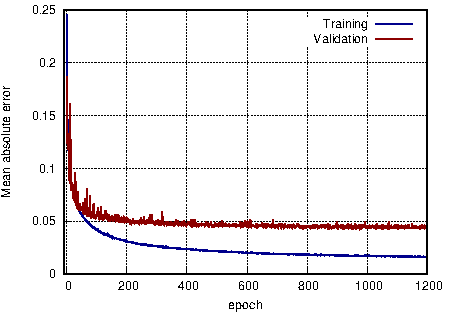
\includegraphics[width=0.9\columnwidth]{figure/training_history.pdf}
\caption{Plot of the training and validation loss function (MAE) versus the training epoch.}
\label{fig:training-history}
\end{figure}

\begin{table}[htbp!]
\centering
\caption{Statistics of the 10-fold cross validation. The mean value and standard deviation of the mean absolute error (MAE) and the root mean square error (RMSE) over 10 runs is given for each of the 3 sets used.}
\begin{tabular*}{\columnwidth}{@{\extracolsep{\fill}} l c c}
\hline
\hline\noalign{\smallskip}
Set        &      MAE         &       RMSE       \\
\noalign{\smallskip}\hline\noalign{\smallskip}
Training   & ~9.4 $\pm$ 0.9 & 18.3 $\pm$ 1.9 \\
Validation & 27.8 $\pm$ 0.7 & 57.8 $\pm$ 2.0 \\
Testing    & 28.1 $\pm$ 0.7 & 58.4 $\pm$ 1.9 \\
\noalign{\smallskip}\hline
\hline
\end{tabular*}
\label{table:crossval}
\end{table}

\begin{table*}[t]
\centering
\caption{Evaluation of the performance of group contribution model\cite{2007Stein}, CNN model\cite{2019Matyushin}, and the model described in this article for selected chemical functionalities for the (unitless) \kovats retention index. The column labelled $N$ indicate the number of data used in computing the mean ($\mu$) and sample standard deviation ($s$) of the MAE.}
\begin{tabular*}{0.85\textwidth}{@{\extracolsep{\fill}} l r r r c r r c r r}
\hline
\hline\noalign{\smallskip}
Molecule & & \multicolumn{2}{c}{Group Contribution} && \multicolumn{2}{c}{~~~~~~~CNN~~~~~~~} && \multicolumn{2}{c}{~~~present work~~~} \\
\noalign{\smallskip}\cline{3-4} \cline{6-7} \cline{9-10} \noalign{\smallskip}
type & $N$~~ & $\mu$~~~ & $s$~~~ && $\mu$~~~ & $s$~~~ && $\mu$~~~ & $s$~~~ \\
\noalign{\smallskip}\hline\noalign{\smallskip}
{\bf all compounds} & ~~102761~ & 113.84 & 119.44 &&  38.97 &  57.08 &&  27.74 &  50.00 \\
ether               &  55755~ & 112.60 & 120.21 &&  34.66 &  52.16 &&  22.99 &  43.87 \\
amide               &  24033~ & 119.26 & 112.20 &&  38.75 &  56.73 &&  25.96 &  47.88 \\
contains O          &  92136~ & 114.36 & 119.88 &&  38.03 &  56.90 &&  26.65 &  49.64 \\
hydrocarbon         &   2010~ &  61.67 &  94.10 &&  33.27 &  49.57 &&  27.77 &  46.75 \\
aromatic            &  70501~ & 121.93 & 119.82 &&  42.48 &  59.36 &&  29.68 &  50.95 \\
has a ring          &  79091~ & 125.44 & 125.90 &&  43.37 &  60.77 &&  30.80 &  53.19 \\
contains N          &  51536~ & 124.71 & 119.04 &&  46.78 &  64.90 &&  33.51 &  56.98 \\
aldehyde            &   1176~ & 114.23 & 121.06 &&  45.89 &  55.80 &&  38.66 &  49.55 \\
contains S          &   9707~ & 127.60 & 120.98 &&  52.85 &  71.25 &&  39.87 &  64.53 \\
N heterocycle       &  22382~ & 155.50 & 138.27 &&  61.12 &  75.80 &&  46.49 &  67.99 \\
ketone              &   5611~ & 168.16 & 172.95 &&  60.98 &  80.86 &&  46.94 &  72.89 \\
O heterocycle       &   9488~ & 182.43 & 173.88 &&  63.13 &  73.99 &&  48.28 &  66.49 \\
alcohol             &   7102~ & 141.22 & 153.86 &&  64.01 &  80.56 &&  52.26 &  75.42 \\
carboxylic acid     &   1444~ & 101.78 & 123.98 &&  63.44 &  95.51 &&  56.09 &  94.95 \\
contains P          &    994~ &        &        && 39.64 &  79.09 &&  31.70 &  73.73 \\
\noalign{\smallskip}\hline
\hline
\end{tabular*}

\label{table:comparison1}
\end{table*}


Figure~\ref{fig:training-history} shows the loss function (MAE) as a function of training epoch. It shows a rapid decrease in the error metric followed by a slow drop; improvement in the performance of the model is not significant after a few hundred epochs. Clearly there is overfitting present in the model as the training error is smaller than validation one. This is also shown in Table~\ref{table:crossval}, which describes the result of 10-fold cross-validation. However, the similar values of the validation and testing set errors indicates that using early-stopping with a validation set is effective. Despite overfitting, the errors of the testing set are acceptable.
The small standard deviations of both error metrics over the 10-fold cross-validation procedure indicate that the model fitting is robust.

The model produces an MAE of 28.1 index units and an RMSE of 58.4 index units. This is a modest improvement over the results achieved by a CNN model \cite{2019Matyushin} which has an MAE of 33.2 and an RMSE of 63.0 index units for the test set from an early version of NIST library.
However, the present results were obtained with a data set more than 3 times larger than that work. To compare the two neural network models more rigorously, we implemented and trained the CNN model with the latest NIST 20 data set using Tensorflow. Our implementation achieved an MAE of 44.4 and an RMSE of 74.6 index units in a 10-fold cross-validation test, both of which are larger than those of our MEGNet model.

Both the MEGNet and CNN model achieved significant improvements over the group contribution model with an MAE of 114.3 and an RMSE of 166.5 index units on the NIST 20 data set. These larger errors of the group contribution model are likely due to inadequacies in the methodology and the use of the less powerful ``classical'' machine learning method. A direct comparison of the three models is in Table~ \ref{table:comparison1}. In all the cases presented, the group contribution exhibits the largest error statistics of the three models.
The largest errors in the two neural network models come from molecules with hydroxyl (OH) groups, such as carboxylic acids and alcohols. We are not aware of any systematic bias that would favor one class of compound over another, so this could be a symptom of data with larger uncertainties or lack of data for a certain class of molecules.
However, this may also suggest that there be room for improvement by explicitly considering certain functional groups.


% Summary and conclusions
\section{SUMMARY, CONCLUSIONS, AND FUTURE WORK}

The work described has demonstrated that machine learning using a graph neural network model is a very effective approach to predict the \kovats retention indices. The model requires only information obtainable from a 2D representation of a molecule (for example, a traditional 2D sketch). The model was trained on a diverse set of more than 100000 molecules. The model predicts the KRI with an MAE of 28 and an RMSE of 58 index units versus the experimental data. The performance of the model is better than the recent one using CNN,\cite{2019Matyushin} and significantly better than the widely used model based on the group contribution methodology.\cite{2007Stein}

The success of the methodology has encouraged us to apply it to predicting a wide range of properties of chemical compounds such as normal boiling points, infrared spectra, and mass spectra, using many high-quality data bases available at NIST. If successful, a new scheme that combines these for the identification of compounds could be developed in the future.


\section{ACKNOWLEDGMENT}

The author thanks Dr. Barry I. Schneider, Dr. Thomas C. Allison, Dr. Anthony J. Kearsley, and Dr. Walid Keyrouz for collaborations on this work. This work was supported by a grant from NIST ITL.% Builing the Future Program.


\begin{thebibliography}{1}

\bibitem{1958Kovats}
E. Kov\'ats, ``Gas-chromatographische Charakterisierung organischer Verbindungen. Teil 1: Retentionsindices aliphatischer Halogenide, Alkohole, Aldehyde und Ketone,'' {\it Helv. Chim. Acta.}, vol. 41, no. 7, pp. 1915--1932, 1958.

\bibitem{2019Chen}
C. Chen, W. Ye, Y. Zuo, C. Zheng, and S. P. Ong, ``Graph Networks as a Universal Machine Learning Framework for Molecules and Crystals,'' {\it Chem. Mater.}, vol. 31, no. 9, pp. 3564--3572, 2019.

\bibitem{2020Wu}
Z. Wu, S. Pan, F. Chen, G. Long, C. Zhang, and P. S. Yu, ``A Comprehensive Survey on Graph Neural Networks,'' {\it IEEE Transactions on Neural Networks and Learning Systems}, vol. 32, no. 1, pp. 4--24, 2020.

\bibitem{2018Zhokhov}
A. K. Zhokhov, A. Yu. Loskutov, and I. V. Rybal’chenko, ``Methodological Approaches to the Calculation and Prediction of Retention Indices in Capillary Gas Chromatography,'' {\it J. Anal. Chem.}, vol. 73, no. 3, pp. 207--220, 2018.

\bibitem{2007Stein}
S. E. Stein, V. I. Babushok, R. L. Brown and P. J. Linstrom, ``stimation of {Kov\'ats} Retention Indices Using Group Contribution,'' {\it J. Chem. Inf. Model.}, vol. 47, pp. 975--980, 2007.

\bibitem{2019Matyushin}
D. D. Matyushin, A. Yu. Sholokhova, and A. K. Buryak, ``A Deep Convolutional Neural Network for the Estimation of Gas Chromatographic Retention Indices,'' {\it J. Chromatogr. A}, vol. 1607, pp. 460395, 2019.

\end{thebibliography}


\begin{IEEEbiography}{Chen Qu} is
currently a postdoctoral researcher at National Institute of Standards and Technology, Gaithersburg, MD, USA. He received the Ph.D. degree in theoretical and computational chemistry from Emory University. Much of his work has focused on solving chemistry problems using machine learning. Contact him at cnq1@nist.gov.
\end{IEEEbiography}

\end{document}

